\documentclass[xcolor=dvipsnames]{beamer}
%\documentclass[handout,xcolor=dvipsnames]{beamer}

% == Packages for beamer
\usepackage{xcolor}
\usepackage{graphicx}
\usepackage{fancybox}
\usepackage{hyperref}
\usepackage{amsmath,amssymb,amsfonts,bm}
\usepackage{wasysym}
\usepackage{colortbl}
\usepackage{booktabs}
\usepackage[english]{babel}
\usepackage{times}
\usepackage[T1]{fontenc}
\usepackage{multirow}

% == Other Packages
\usepackage{rotating}
\usepackage{latexsym}
\usepackage{ulem}
\usepackage{tikz}
\usetikzlibrary{positioning,arrows.meta}

% == theme & colors
\usetheme{Warsaw}
\usepackage{helvet}
\definecolor{someblue}{rgb}{0,.1,0.8}
\definecolor{dgreen}{rgb}{0,.6,0.8}
\useoutertheme{infolines}

% == New Commands
\newcommand\spacingset[1]{\renewcommand{\baselinestretch}{#1}\small\normalsize}
\renewcommand\r{\right}
\renewcommand\l{\left}
\newcommand\makegaps{\addtolength{\itemsep}{.25\baselineskip}}
\newcommand\makebiggaps{\addtolength{\itemsep}{.5\baselineskip}}

% = For stats & econometrics
\renewcommand{\epsilon}{\varepsilon}
\newcommand\E{\mathbb{E}}
\newcommand\V{\mathbb{V}}
\newcommand{\Var}{\mathrm{Var}}
\newcommand{\Cov}{\mathrm{Cov}}
\newcommand\indep{\protect\mathpalette{\protect\independenT}{\perp}}
\def\independenT#1#2{\mathrel{\rlap{$#1#2$}\mkern2mu{#1#2}}}

\newtheorem{iass}{Identification Assumption}
\newtheorem{ires}{Identification Result}

\title[SOO I]{Selection on Observables I: The Assumption}
\subtitle[ ]{Stat 256, Spring 2026}
\author[Hazlett]{Chad Hazlett}
\institute[UCLA]{UCLA\\[1ex]
  \texttt{chazlett@ucla.edu}
}
\date{}

\begin{document}

\begin{frame}
  \titlepage
\end{frame}


%% =====================================================================
\section{From Experiments to Observational Studies}
%% =====================================================================

\begin{frame}{Where we are}
\small
\onslide<1-> \textcolor{Blue}{Unit 1}: DAGs, d-separation, backdoor criterion --- a \textit{graphical} language for identification.\\[4pt]

\onslide<2-> \textcolor{Blue}{Unit 2}: Potential outcomes, experiments --- ignorability from randomization gives
$$\tau_{\text{ATE}} = \E[Y_i \mid D_i\!=\!1] - \E[Y_i \mid D_i\!=\!0].$$

\onslide<3-> \textcolor{Blue}{Unit 3 (now)}: Observational studies. No randomization. We need an \textit{assumption} to recover causal effects by conditioning on observed $X$.\\[4pt]

\onslide<4-> Today: the assumption, its two languages (CI $\leftrightarrow$ backdoor), and stratification as the first estimator. Wednesday: matching, weighting, regression.
\end{frame}


\begin{frame}{The First Commandment of Causal Inference}
\small
\onslide<1->
\begin{center}
\large \textit{No causal claim without a supporting}\\[4pt]
\textit{causal assumption.}
\end{center}

\bigskip
\onslide<2-> The assumption does the identifying work. The estimator is secondary.\\

\medskip
\onslide<3-> Corollaries:
\begin{itemize}
\footnotesize
\item<3-> ``We used matching'' is not a causal argument.
\item<4-> ``We controlled for everything we could think of'' is not a causal argument.
\item<5-> ``We used machine learning to pick controls'' is not a causal argument.
\end{itemize}

\bigskip
\onslide<6-> All of these are \textit{estimation} choices. They serve a causal claim only if the underlying \textit{identification assumption} is credible.
\end{frame}


\begin{frame}{Setting}
\small
\onslide<1->
\begin{itemize}
\item Units: $i = 1, \ldots, N$
\item Treatment: $D_i \in \{0,1\}$, \textbf{not} randomly assigned
\item Potential outcomes: $Y_{0i}$, $Y_{1i}$; observed $Y_i = D_i Y_{1i} + (1-D_i) Y_{0i}$
\item Pre-treatment covariates: $X_i$ (a vector)
\item Quantity of interest: $\tau_{\text{ATE}} = \E[Y_{1i} - Y_{0i}]$ (or $\tau_{\text{ATT}}$)
\end{itemize}

\bigskip
\onslide<2-> A covariate $X$ is a \textbf{confounder} if it is associated with both $D$ and the potential outcomes $Y_d$.
\end{frame}


%% =====================================================================
\section{Conditional Ignorability}
%% =====================================================================

\begin{frame}{The Assumption: Conditional Ignorability}
\small
\onslide<1->
\begin{iass}[Conditional Ignorability / Selection on Observables]
$$\{Y_{1i}, Y_{0i}\} \indep D_i \mid X_i$$
\end{iass}

\onslide<2-> Many names for the same thing:
\begin{itemize}
\footnotesize
\item Conditional ignorability (CI)
\item Selection on observables (SOO)
\item No unmeasured confounders
\item Conditional exchangeability
\item ``Backdoor criterion satisfied by $X$'' (DAG language)
\end{itemize}

\bigskip
\onslide<3-> Read it as: \textit{among units with the same $X$, treatment assignment is as good as random.}
\end{frame}


%% =====================================================================
\section{Why CI = Backdoor}
%% =====================================================================

\begin{frame}{CI and the backdoor criterion: two languages, one object}
\small
\onslide<1-> In Unit 1 we said: if $X$ satisfies the backdoor criterion relative to $(D,Y)$ in a DAG, the effect of $D$ on $Y$ is identified by adjusting for $X$:
$$P(Y \mid do(D\!=\!d)) = \sum_x P(Y \mid D\!=\!d, X\!=\!x)\,P(X\!=\!x).$$

\onslide<2-> In PO language we just said CI means $\{Y_{1i}, Y_{0i}\} \indep D_i \mid X_i$.\\[4pt]

\onslide<3-> \textcolor{Blue}{Claim}: these are the \textit{same statement}, written in different alphabets.  Let's see why.
\end{frame}


\begin{frame}{Informal argument}
\small
\onslide<1-> Backdoor-satisfying $X$ blocks all non-causal paths from $D$ to $Y$:
\begin{itemize}
\footnotesize
\item<2-> Any association between $D$ and $Y$ that remains \textit{within a stratum of $X$} can only come from the causal arrow $D \to Y$.
\item<3-> Equivalently: within a stratum of $X$, treatment carries no information about the potential outcomes beyond its causal effect.
\item<4-> That is conditional ignorability: $\{Y_{1i}, Y_{0i}\} \indep D_i \mid X_i$.
\end{itemize}

\bigskip
\onslide<5-> So ``block the backdoors'' (DAG side) and ``$D$ is as-if randomized within strata of $X$'' (PO side) say the same thing.  To make this precise we need to be able to \textit{see} potential outcomes on the graph.
\end{frame}


\begin{frame}{View 1: the test graph $G_{\underline{D}}$}
\vspace{-4pt}
\small
\onslide<1-> Take your DAG. Delete all arrows \textit{out of} $D$. Call this $G_{\underline{D}}$.\\[4pt]
\onslide<2->
\begin{columns}[T]
\begin{column}{.5\textwidth}
\begin{center}
\textbf{Original DAG}\\[4pt]
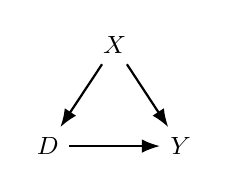
\begin{tikzpicture}[->,>=Latex,thick,node distance=1.6cm,
  every node/.style={font=\small}]
\node (X) {$X$};
\node (D) [below left= 0.8cm and 0.3cm of X] {$D$};
\node (Y) [below right=0.8cm and 0.3cm of X] {$Y$};
\draw (X) -- (D);
\draw (X) -- (Y);
\draw (D) -- (Y);
\end{tikzpicture}
\end{center}
\end{column}
\begin{column}{.5\textwidth}
\begin{center}
\textbf{$G_{\underline{D}}$: delete $D \to Y$}\\[4pt]
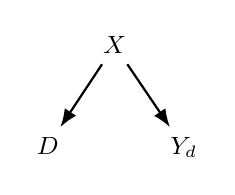
\begin{tikzpicture}[->,>=Latex,thick,node distance=1.6cm,
  every node/.style={font=\small}]
\node (X) {$X$};
\node (D) [below left= 0.8cm and 0.3cm of X] {$D$};
\node (Y) [below right=0.8cm and 0.3cm of X] {$Y_d$};
\draw (X) -- (D);
\draw (X) -- (Y);
\end{tikzpicture}
\end{center}
\end{column}
\end{columns}

\medskip
\onslide<3-> In $G_{\underline{D}}$, the only way $D$ and $Y$ associate is through $X$.  So: $D \indep Y \mid X$ in $G_{\underline{D}}$.\\[4pt]

\onslide<4-> $G_{\underline{D}}$ is a ``null graph'': $Y= Y_1 = Y_0$. So we actually have:
$$Y_d \indep D \mid X.$$
\onslide<5-> Thus conditional ignorability is certified.\\
\end{frame}


\begin{frame}{View 2: SWIGs (Richardson \& Robins, 2013)}
\small
\onslide<1-> The core difficulty is that we need to reference both the realized $D$ and the potential outcome $Y_d$ even when $d \neq D$.\\
\medskip
\onslide<2-> The SWIG (single world intervention graph) does just that:
\begin{columns}[T]
\begin{column}{.5\textwidth}
\begin{center}
\textbf{DAG}\\[4pt]
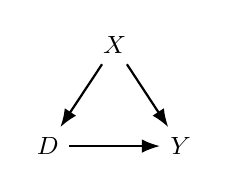
\begin{tikzpicture}[->,>=Latex,thick,node distance=1.6cm,
  every node/.style={font=\small}]
\node (X) {$X$};
\node (D) [below left= 0.8cm and 0.3cm of X] {$D$};
\node (Y) [below right=0.8cm and 0.3cm of X] {$Y$};
\draw (X) -- (D);
\draw (X) -- (Y);
\draw (D) -- (Y);
\end{tikzpicture}
\end{center}
\end{column}
\begin{column}{.5\textwidth}
\begin{center}
\textbf{SWIG: intervene $do(D=d)$}\\[4pt]
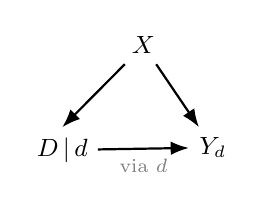
\begin{tikzpicture}[->,>=Latex,thick,node distance=1.6cm,
  every node/.style={font=\small}]
\node (X) {$X$};
\node (D) [below left= 0.8cm and 0.3cm of X] {$D \,|\, d$};
\node (Y) [below right=0.8cm and 0.3cm of X] {$Y_d$};
\draw (X) -- (D.north);
\draw (X) -- (Y);
\draw (D) -- (Y) node[midway,below] {\scriptsize\textcolor{gray}{via $d$}};
\end{tikzpicture}
\end{center}
\end{column}
\end{columns}

\medskip
\onslide<3-> The ``$D \mid d$'' node splits: the left side is the ``natural'' $D$ you observe; the right side is the set value $d$ that flows into $Y_d$.\\[4pt]

\onslide<4->  You can see CI directly as d-separation of $D$ from $Y_d$ in the SWIG: $$Y_d \indep D \mid X$$
\end{frame}


\begin{frame}{Formal statement, with a nod to the literature}
\footnotesize
\onslide<1-> \textbf{Theorem (backdoor/adjustment criterion $\Rightarrow$ CI)}. If $X$ satisfies the backdoor criterion relative to $(D,Y)$ in a DAG $G$, then in any SCM consistent with $G$,
$$Y_d \indep D \mid X \quad \text{for each } d.$$

\medskip
\onslide<2-> \textbf{References for more}:
\begin{itemize}
\footnotesize
\item Pedagogical/informal but nice: \textit{What If}, ch.\ 7.
\item Direct, formal: Pearl, Glymour \& Jewell (2016), \textit{Primer}, Thm 4.3.1: backdoor-satisfying $Z \Rightarrow Y_x \indep X \mid Z$.
\item Also formal: Shpitser, VanderWeele \& Robins (2010), Thm 4 states adjustment criterion and ties that to CI on their ``counterfactual graph.''\footnote{These are like SWIGs but rather than splitting nodes, you show multiple copies of the graph, with and without intervention, with fused exogenous variables. Similar to ``twin networks'' we will mention later.}
%\item Richardson \& Robins (2013), ``Single world intervention graphs: a primer'': the PO-from-DAG semantics (FFRCISTG) under which the SWIG reasoning is licensed.
\end{itemize}
\end{frame}


% \begin{frame}{Upshot}
% \onslide<1-> Take-home message: two languages, one object.\\

% % \small
% % \onslide<1->
% % \begin{center}
% % \begin{tabular}{@{} l c l @{}}
% % \toprule
% % \textbf{DAG language} & $\Leftrightarrow$ & \textbf{PO language}\\
% % \midrule
% % $X$ satisfies backdoor & & $\{Y_{1i},Y_{0i}\} \indep D_i \mid X_i$\\
% % adjustment formula & & stratification estimator\\
% % $\sum_x P(Y\mid D,X\!=\!x)P(X\!=\!x)$ & & $\sum_x \E[Y\mid D,X\!=\!x] \Pr(X\!=\!x)$\\
% % \bottomrule
% % \end{tabular}
% % \end{center}

% \bigskip

% \onslide<1-> Same object, two notations. Use whichever is easier to think in:

% \begin{itemize}
% \footnotesize
% \item<2-> DAG is good for \textit{choosing} $X$: What blocks the backdoors? What traps must I avoid?
% \item<3-> PO is good for \textit{stating} the estimand and the estimator crisply.
% \end{itemize}
% \medskip
% \onslide<3-> The rest of today works in PO language.
% \end{frame}


%% =====================================================================
\section{Credibility and Positivity}
%% =====================================================================

\begin{frame}{What would make CI true?}
\small
\onslide<1-> \textbf{CI is a strong assumption.}  It says that all confounders are observed and included in $X$.\\[6pt]

\onslide<2-> Credibility depends on the \textit{story}: what determined treatment and outcome, and have you measured all of it?\\[4pt]

\onslide<3-> What sorts of stories work?
\begin{itemize}
  \item<3-> \textbf{Design}: a conditionally randomized experiment (e.g., block-randomized with different treatment probabilities per stratum). Then CI holds by construction.\\[2pt]
  \item<3-> \textbf{Observational}: you must \textit{argue} that $X$ captures all common causes of $D$ and $Y$.  Substantive knowledge, not statistical testing.
\end{itemize}

\bigskip
\onslide<4-> CI is \textbf{not verifiable from the data}.  No amount of checking observed covariates can rule out unobserved confounders.
\end{frame}


\begin{frame}{Common Support / Positivity}
\small
\onslide<1-> CI alone is not enough. Another ``identification-like'' assumption: 
\begin{iass}[Common Support / Overlap]
$$0 < \Pr(D_i = 1 \mid X_i = x) < 1 \quad \text{for all } x \text{ in the support of } X.$$
\end{iass}

\onslide<2-> Weaker version for ATT: only need $\Pr(D = 1 \mid X) < 1$ (need controls for every treated stratum, but not vice versa).\\[4pt]
\medskip
\onslide<3-> This is somewhat ill-defined:
\footnotesize
\begin{itemize}
\item What if $X$ is continuous?  Then we are assuming some unclear form of smoothness in $\Pr(D\mid X)$
\item ``Practical'' positivity violations: some strata may lack observed treated or control units, even if they are not zero probability. 
\item An alternative: abandon common support and worry instead about reasoned uncertainty in each $\E[Y_d|X]$ as we move away from supporting data.
\end{itemize}

\end{frame}


%% =====================================================================
\section{Identification under CI}
%% =====================================================================

\begin{frame}[t]{Identification of the ATE under CI}
\small
\onslide<1-> \textcolor{Blue}{Quantity}: $\tau_{\text{ATE}} = \E[Y_{1i} - Y_{0i}]$\\[6pt]

\onslide<2-> \textcolor{Blue}{Step 1}: within a stratum of $X$, CI gives an ``experiment'':
\footnotesize
\begin{align*}
\E[Y_{1i} - Y_{0i} \mid X\!=\!x]
  &= \E[Y_{1i} \mid X\!=\!x] - \E[Y_{0i} \mid X\!=\!x]\\
  &\stackrel{\text{CI}}{=} \E[Y_{1i} \mid D\!=\!1, X\!=\!x] - \E[Y_{0i} \mid D\!=\!0, X\!=\!x]\\
  &\stackrel{\text{consistency}}{=} \E[Y_i \mid D\!=\!1, X\!=\!x] - \E[Y_i \mid D\!=\!0, X\!=\!x].
\end{align*}
\medskip
\onslide<3-> \textcolor{Blue}{Step 2}: put the strata back together using $\Pr(X)$:
\footnotesize
\begin{align*}
\tau_{\text{ATE}}
  &= \E_X\!\big[\E[Y_{1i} - Y_{0i} \mid X]\big]\\
  &= \sum_x \big(\E[Y_i \mid D\!=\!1, X\!=\!x] - \E[Y_i \mid D\!=\!0, X\!=\!x]\big)\,\Pr(X\!=\!x).
\end{align*}

\small
\onslide<4-> The RHS is fully observable (given positivity), so the ATE is \textbf{identified}.\\[6pt]

\onslide<5-> \centering{Exactly what you did with the adjustment formula.\footnote{Here we are asking for $P(Y \mid do(D=1))-P(Y\mid do(D=0))$ at once, instead of each $P(Y\mid do(D))$.}}
\end{frame}


%% =====================================================================
\section{Cochran: Smoking and Mortality}
%% =====================================================================

\begin{frame}{Example: Smoking and Mortality (Cochran 1968)}
\small
Unadjusted death rates per 1{,}000 person-years:

\begin{center}
\begin{tabular}{@{} l c c c @{}}
\toprule
 & Canada & U.K. & U.S.\\
\midrule
Non-smokers     & 20.2 & 11.3 & 13.5 \\
Cigarette only  & 20.5 & 14.1 & 13.5 \\
Cigars/pipes    & 35.5 & 20.7 & 17.4 \\
\bottomrule
\end{tabular}
\end{center}

\bigskip
\onslide<2-> Pipe/cigar smokers die at much higher rates.  Causal effect of smoking?

\onslide<3-> \medskip
Or could something else explain this?
\end{frame}


\begin{frame}{The Confounder: Age}
\small
Mean ages by smoking group:

\begin{center}
\begin{tabular}{@{} l c c c @{}}
\toprule
 & Canada & U.K. & U.S.\\
\midrule
Non-smokers     & 54.9 & 49.1 & 57.0 \\
Cigarette only  & 50.5 & 49.8 & 53.2 \\
Cigars/pipes    & 65.9 & 55.7 & 59.7 \\
\bottomrule
\end{tabular}
\end{center}

\bigskip
\onslide<2-> Pipe/cigar smokers are \textit{much older} on average.\\
\medskip
\onslide<3-> Age is associated with both smoking type and death rate --- it is a confounder.  Can we adjust for it?
\end{frame}


\begin{frame}{Subclassification Reveals the Effect}
\small
\onslide<1-> Fabricated data inspired by the U.S.\ figures (death rates per 1{,}000 person-years):

\begin{center}
\footnotesize
\begin{tabular}{@{} l c c c c c @{}}
\toprule
Age group & Rate (Cig) & Rate (Non) & Effect & $N$ (Cig) & $N$ (Non) \\
\midrule
$<45$    & 5  & 3  & $+2$  & 40 & 10 \\
$45$--$54$ & 10 & 5  & $+5$  & 30 & 20 \\
$55$--$64$ & 20 & 10 & $+10$ & 20 & 30 \\
$65+$    & 45 & 23 & $+22$ & 10 & 40 \\
\midrule
Pooled   & 13.5 & 13.5 & $0$ & 100 & 100 \\
\bottomrule
\end{tabular}
\end{center}

\onslide<2-> Within every age group, smokers die at higher rates.  But the pooled difference is \textbf{zero} --- because smokers are younger.\\

\medskip
\onslide<3-> Subclassification (each age stratum has $N_j = 50$):
$$\hat\tau_{\text{ATE}} = \frac{1}{4}\big(2 + 5 + 10 + 22\big) = 9.75$$

\onslide<4-> The confounding hid an effect of nearly 10 deaths per 1{,}000 person-years.
\end{frame}


\begin{frame}{The Most Important Slide}
\small
\onslide<1-> Pause and ask:
\begin{itemize}
\item<2-> What \textbf{assumption} did we need to interpret this causally?
\medskip
\item<3-> State it as CI: $\{Y_{1i}, Y_{0i}\} \indep D_i \mid X_i$. What is $X$ here?
\medskip
\item<4-> State it in ``unobserved confounders'' language.
\medskip
\item<5-> Do you believe it?  What unmeasured $U$ could violate CI?
\medskip
\item<6-> Can you \textit{test} CI with data?  What can you test?
\end{itemize}

\bigskip
\onslide<7-> \textbf{This} is the hard part --- not the estimator.
\end{frame}


%% =====================================================================
\section{Post-treatment Conditioning, and Estimation Preview}
%% =====================================================================

\begin{frame}{Don't Condition on Post-treatment Variables}
\small
\onslide<1-> You already know why: 
\begin{itemize}
\footnotesize
\item<2-> \textbf{Selection bias}: if you restrict to a subset of the data defined by a post-treatment variable, you may be selecting on a collider, inducing an association between $D$ and the confounder that wasn't there before, breaking the randomization. 
\item<3-> \textbf{Mediation ``bias''} (or changing the estimand): if you control for a variable that is on the causal pathway from $D$ to $Y$, you are blocking part of the causal effect you are trying to estimate, which can lead to an underestimate of the total effect.
\end{itemize} 

\onslide<4-> What we understood simply as collider bias before should be visible to you as a violation of CI. Conditioning on some $Z$ with $D \rightarrow Z \leftarrow U \rightarrow Y$ 
\begin{itemize}
\footnotesize
\item  changes the distribution of $Y_d$ (because of the $U$),
\item and does so differently for the treated vs. control (because of the $D$), so you lose the $Y_d \indep D$ you thought you had.
\end{itemize}
\end{frame}


\begin{frame}{Estimation under CI: the idea}
\small
\onslide<1-> The ID result says: compute treatment effects \textit{within strata of $X$}, then average over the population distribution of $X$.\\[4pt]
\medskip
\onslide<2-> \textbf{Subclassification} (stratification) does this literally when $X$ is discrete:
\begin{enumerate}
\footnotesize
\item Divide units into $J$ strata defined by $X$.
\item Within-stratum DIM: $\hat\tau_j = \bar Y_{1j} - \bar Y_{0j}$.
\item Average: $\hat\tau_{\text{ATE}} = \sum_{j=1}^J \frac{N_j}{N}\, \hat\tau_j$.
\end{enumerate}

\medskip
\onslide<3-> No modeling.  Simply the  adjustment formula from the DAG (twice).\\[4pt]

\onslide<4-> \textbf{But}: breaks down when $X$ has many components or continuous entries --- most strata have 0 treated or 0 controls (curse of dimensionality).\\
\bigskip
\onslide<5-> \textbf{Next time}: matching, propensity scores, weighting, regression --- all trying to do the same thing when literal stratification fails.
\end{frame}


\begin{frame}{Takeaways}
\small
\begin{itemize}
\item<1-> \textbf{CI/SOO is an assumption, not a procedure.}  ``No unmeasured confounders'' is a strong, unverifiable claim about the world.
\medskip
\item<2-> \textbf{CI and the backdoor criterion are the same statement} in different alphabets.  Adjustment formula $=$ stratification estimator.
\medskip
\item<3-> \textbf{Credibility comes from the story}, not the data.
\medskip
\item<4-> \textbf{Positivity} is a separate, ID-like assumption, but can be murky.
\medskip
\item<5-> \textbf{Don't condition on post-treatment variables.}
\medskip
\item<6-> \textbf{Once you believe CI}, the estimation question (matching, weighting, regression) is secondary.  We turn to that next.
\end{itemize}
\end{frame}


%% =====================================================================
\section{Logistics}
%% =====================================================================

\begin{frame}{Reminder: Advanced Topic Presentations}
\small
\textbf{Due today}: submit \textit{group} (2--3 students) and \textit{top 3 topics} (ranked) using the google form sent via BruinLearn.\\[6pt]

\onslide<2->
\begin{itemize}
\footnotesize
\item See \texttt{PresentationAssignment.pdf} on the course site for the topic list.
\item Stick around or email me if you want to talk about this or help find group members. 
\end{itemize}
\end{frame}


\end{document}
